\section{Listener behaviours in collective decision-making} \label{sect:listener_models}

\subsection*{Passive Model}
Having proposed several ways for the speaker to construct an argument, we now consider the strategies that listener agents may employ to update their beliefs. Drawing inspiration from the FJ model~\cite{Friedkin1999SocialChange}, we define an update rule that maintains an element of the agents previous beliefs as well as assimilating the new information. This rule is given by

\begin{equation} \label{eq:BU_update_rule}
    \underline{\mathbf{P}}^{t+1}_l = \alpha \cdot \underline{\mathbf{P}}^{t}_l + (1 - \alpha) \cdot  \frac{\underline{\mathbf{A}} \odot \underline{\mathbf{P}}^t_l}{\underline{\mathbf{A}} \cdot \underline{\mathbf{P}}^t_l}
\end{equation}

where $\alpha$ is a parameter in the interval $[0, 1]$ that governs the responsiveness of an agent to new information~\cite{Hegselmann2002OpinionSimulation}. Here, the set of asserted states $\mathbf{A}$ is translated into a $1 \times n$ column vector $\underline{\mathbf{A}}$. In Hegselmann's work $\alpha$ differs depending upon how reliable the population believes the speaker to be, while here, it is consistent across all agents. Furthermore, $\odot$ denotes the elementwise or Haramaard product~\cite{Johnson1990MatrixApplications}. The final component of this equation is the agent's posterior distribution given $\mathbf{A}$. This final term conditions the speaker's argument $\mathbf{A}$ on the listener's original beliefs. If this conditioning were to become undefined by the denominator equalling zero, the listener's beliefs would no longer sum to 1. Such an agent would be described as incoherent and would no longer be functional~\cite{Lee2018CombiningConsensus}. An agent can only become incoherent when the listener's probability for the assertion $P_L(\mathbf{A}) = 0$. Therefore, in this case, the listener simply does not update.

It should be noted that the Open model must be treated differently. The above equation is tailored toward arguments of binary vectors, where the Open model broadcasts distributions. Therefore, when the Open model is applied, the equation becomes,

\begin{equation} 
    \underline{\mathbf{P}}^{t+1}_l = \alpha \cdot \underline{\mathbf{P}}^{t}_l + (1 - \alpha) \cdot \underline{\mathbf{P}_s^t} 
\end{equation}


\subsection*{Discerning Model}

In the Passive model, the listener does not possess the ability to disregard any information it receives; it will always update its beliefs based on new information. To address this, the Discerning model requires that when the listener reverses the process that is used to create the argument on its own beliefs, the same condition must be met. Consider the following example for illustration. 

Let the speaker broadcast $\underline{\mathbf{A}} = \begin{bmatrix}
    1,
    0,
    1
\end{bmatrix}^T$
and let the listener's beliefs
$\underline{\mathbf{P}}^t_l = \begin{bmatrix}
    0.6,
    0.15,
    0.25
\end{bmatrix}^T$. If this argument was constructed with the Bottom Up method with a threshold $\gamma = 0.4$, the listener compares the argument elementwise with its own beliefs. It finds that $p_1 > \gamma$ passing the requirement, $p_2$ is not asserted so is not considered, and finally $p_3 < \gamma$. $H_3$ seems unlikely to the listener, therefore it rejects the assertion outright, and refuses to update. Similarly, if the argument was created with the Top Down model with a threshold $\gamma = 0.8$, then the listener takes the dot product of $\underline{\mathbf{A}}$ and $\underline{\mathbf{P}}_l^t$. Here, this returns a value of $0.85$ which is greater than $\gamma$ so the listener accepts the argument and updates accordingly. This discernment is only possible in the Bottom Up and Top Down models as they involve a specified criterion that the argument must meet to be transmitted.


\subsection*{Backfiring Model}

The Discerning model is simple in that, should the listener disagree with the argument, it does not update its beliefs whatsoever. While this trait can be found in human behaviour, it is also plausible that an argument may backfire. For an individual who has lost their temper, it is unlikely that the suggestion ``calm down'' will achieve its intended aim, instead serving only to worsen that individual's mood. In this Backfiring model, the argument will be rejected if the same conditions as the Discerning model are met. Should this happen, the listener will update their beliefs using $\mathbf{A}^c$, shown below

\begin{equation} \label{eq:Backfiring_update_rule}
    \underline{\mathbf{P}}^{t+1}_l = \alpha \cdot \underline{\mathbf{P}}^{t}_l + (1 - \alpha) \cdot  \frac{\underline{\mathbf{A}}^c \odot \underline{\mathbf{P}}^t_l}{\underline{\mathbf{A}}^c \cdot \underline{\mathbf{P}}^t_l}
\end{equation}

It is expected that both the Discerning and Backfiring models will cause divisions in the population, creating regions in which agents are incapable of responding to an argument. This is due to the fact that, as soon as there is a threshold an argument must meet to be accepted, there will be arguments that do not meet it, limiting the ability of agents with strongly opposing views to listen to each other. 



\subsection*{Acclimatisation Model}

The Acclimatisation model aims to capture the loss of na\"{i}vety of the listeners; the more arguments they hear, the less they respond to them. This model uses \cref{eq:BU_update_rule}, with a minor alteration to the significance of $\alpha$. Here, it is a function of the total number of arguments that the agent has received, even if they are repetitious. This number is referred to as $\tau$. $\alpha$ is given by

\begin{equation}
    \alpha (\tau) = 1 - (1 - \alpha_0) e^{-\phi \tau}
\end{equation}

where $\alpha_0$ is the initial value of $\alpha$ and $\phi$ is the rate at which the agents become acclimatised. This equation dictates that the impact of the first arguments an agent receives is significant, while the latter arguments are less and less impactful. This can be seen in \cref{fig:stubbornness_curve}. 

\begin{figure}[H]
    \centering
    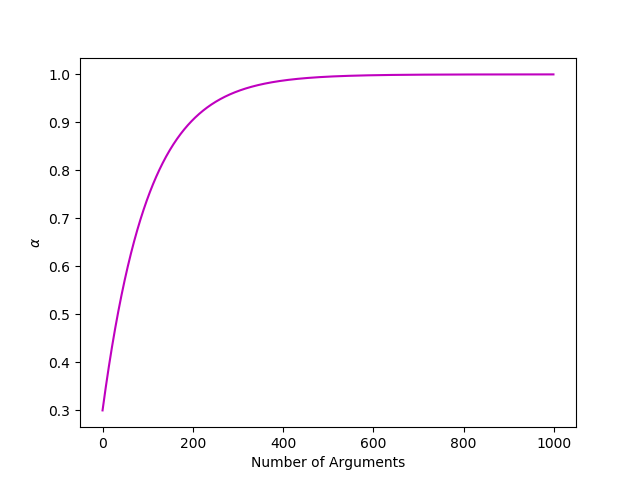
\includegraphics[width=0.49\textwidth]{Images/Misc/Stubbornness.png}
    \caption{A graph to show the rate at which agents change the importance they place on new information in the Acclimatisation Model. \textit{Using $\alpha_0 = 0.3, \phi = 0.01$}}
    \label{fig:stubbornness_curve}
\end{figure}

Here, as $\tau$ increases, so does $\alpha$, meaning that the update rule

\begin{equation} 
    \underline{\mathbf{P}}^{t+1}_l = \alpha(\tau) \cdot \underline{\mathbf{P}}^{t}_l + (1 - \alpha(\tau)) \cdot  \frac{\underline{\mathbf{A}} \odot \underline{\mathbf{P}}^t_l}{\underline{\mathbf{A}} \cdot \underline{\mathbf{P}}^t_l}
\end{equation}

places decreasing weight on new information, and that as $\tau \rightarrow \infty, \alpha \rightarrow 1$. At this point, the update rule becomes

\begin{equation} 
    \underline{\mathbf{P}}^{t+1}_l = \underline{\mathbf{P}}^{t}_l 
\end{equation}